%%%%%%%%%%%%%%%%%%%%%%%%%%%%%%%%%%%%%%%%%
% University Assignment Title Page 
% LaTeX Template
% Version 1.0 (27/12/12)
%
% This template has been downloaded from:
% http://www.LaTeXTemplates.com
%
% Original author:
% WikiBooks (http://en.wikibooks.org/wiki/LaTeX/Title_Creation)
%
% License:
% CC BY-NC-SA 3.0 (http://creativecommons.org/licenses/by-nc-sa/3.0/)
% 
% Instructions for using this template:
% This title page is capable of being compiled as is. This is not useful for 
% including it in another document. To do this, you have two options: 
%
% 1) Copy/paste everything between \begin{document} and \end{document} 
% starting at \begin{titlepage} and paste this into another LaTeX file where you 
% want your title page.
% OR
% 2) Remove everything outside the \begin{titlepage} and \end{titlepage} and 
% move this file to the same directory as the LaTeX file you wish to add it to. 
% Then add \input{./title_page_1.tex} to your LaTeX file where you want your
% title page.
%
%%%%%%%%%%%%%%%%%%%%%%%%%%%%%%%%%%%%%%%%%
%\title{Title page with logo}
%----------------------------------------------------------------------------------------
%	PACKAGES AND OTHER DOCUMENT CONFIGURATIONS
%----------------------------------------------------------------------------------------

\documentclass[12pt]{article}
\usepackage[margin=1in]{geometry}
\usepackage[english]{babel}
\usepackage[utf8x]{inputenc}
\usepackage{amsmath}
\usepackage{bm}
\usepackage{graphicx}
\usepackage[colorinlistoftodos]{todonotes}
\usepackage{natbib}


\usepackage[hidelinks]{hyperref}
\begin{document}

\begin{titlepage}

\newcommand{\HRule}{\rule{\linewidth}{0.5mm}} % Defines a new command for the horizontal lines, change thickness here

\center % Center everything on the page
 
%----------------------------------------------------------------------------------------
%	HEADING SECTIONS
%----------------------------------------------------------------------------------------

\textsc{\LARGE Ukrainian Catholic University}\\[1cm] % Name of your university/college
\textsc{\Large Applied Sciences Faculty}\\[0.5cm] % Major heading such as course name
\textsc{\large Data Science Master Programme}\\[0.5cm] % Minor heading such as course title

%----------------------------------------------------------------------------------------
%	TITLE SECTION
%----------------------------------------------------------------------------------------

\HRule \\[0.4cm]
{ \huge \bfseries Kernel Principal Component Analysis and its Applications}\\[10pt]
{\Large \bfseries Project report}\\[0.4cm] % Title of your document
\HRule \\[1cm]
 
%----------------------------------------------------------------------------------------
%	AUTHOR SECTION
%----------------------------------------------------------------------------------------


% If you don't want a supervisor, uncomment the two lines below and remove the section above
\Large \emph{Authors:}\\
Irynei \textsc{Baran}\\Hanna \textsc{Pylieva}\\[1cm] % Your name

%----------------------------------------------------------------------------------------
%	DATE SECTION
%----------------------------------------------------------------------------------------

{\large \today}\\[2cm] % Date, change the \today to a set date if you want to be precise

%----------------------------------------------------------------------------------------
%	LOGO SECTION
%----------------------------------------------------------------------------------------


\includegraphics[height=4cm]{img/UCU-Apps.png}\\[1cm] % Include a department/university logo - this will require the graphicx package
 
%----------------------------------------------------------------------------------------

\vfill % Fill the rest of the page with whitespace

\end{titlepage}


\begin{abstract}
Principal component analysis (PCA) is a
popular tool for linear dimensionality reduction
and feature extraction. Kernel PCA
is the nonlinear form of PCA, which better
exploits the complicated spatial structure of
high-dimensional features. In this project, we review the basic ideas of PCA, identify its limitations and possible modifications. Then we concentrate on one important extension of PCA - kernel
PCA. We give the detailed explanation of the latter, followed by step-by-step instructions of the algorithm's implementation.  We also provide the source code of kPCA developed by ourselves with comparison of its performance against linear PCA. Finally, we briefly specify the possible applications of kPCA and discuss the method's pros and cons.
\end{abstract}

\section{Principal Component Analysis}
Principal component analysis, or PCA, is a mathematical procedure which is widely used for dimensionality reduction and feature selection. Those applications are achieved by projecting the data orthogonally onto a linear space with lower dimension, known as the principal subspace or feature space, such that the variance of projected data is maximal \citep*{bishop}.

Consider a data set $X$ containing $N$ observations of $D$ features ($D<N$). In order to visualize data or diminish number of features for modeling we want to reduce dimensionality of feature space to $M<D$. Whereas we are interested in most influential features to minimize data losses, that is why our goal is to maximize variance of projected data. The directions on which the data is projected called principal components. They are orthogonal and form coordinate system of subspace $M$ (see on ~\autoref{fig:pr-components}).

\begin{figure}[h]
	\centering
	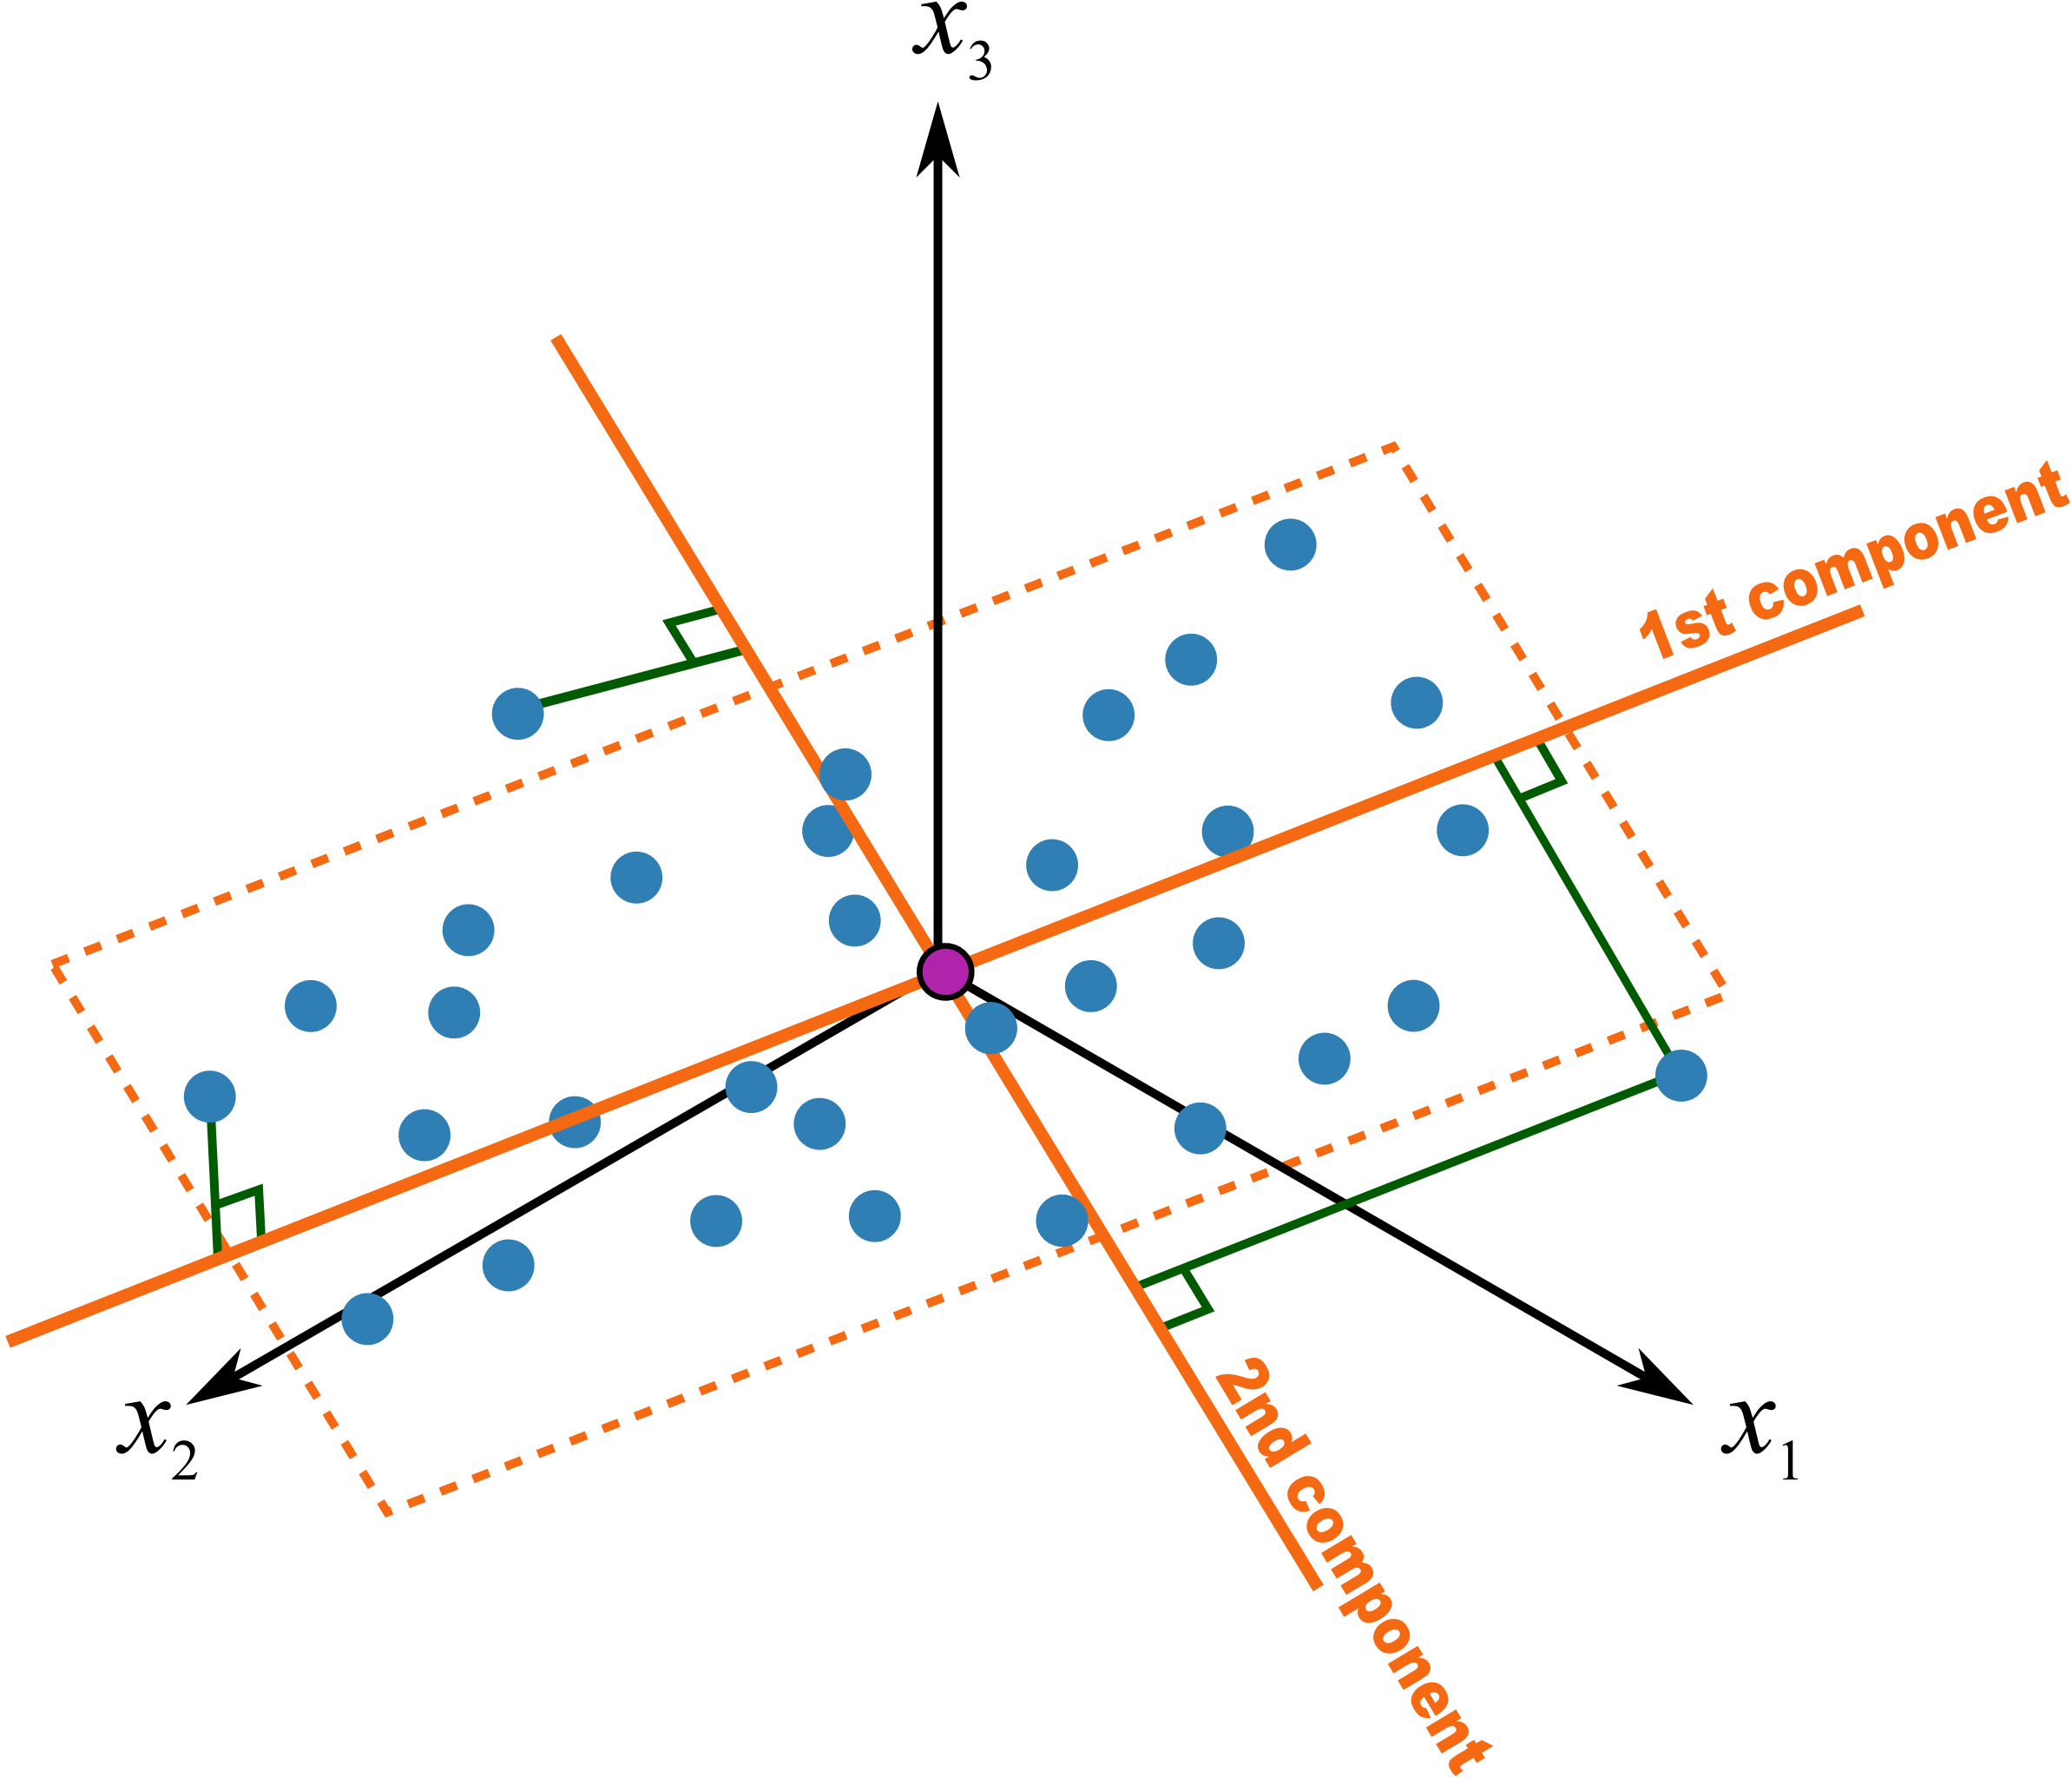
\includegraphics[scale=0.3]{img/geometric-PCA-8-both-components-with-plane.png}
	\caption{\label{fig:pr-components}Principal components}
\end{figure}

\subsection{Finding principal components}
To begin with, consider the projection on $M$ when $dim(M)=1$. Let a unit vector $u_1 \in D$ be the direction of $M$. Then projection of an observation $x_n\in X$ onto $M$ is $u_1^Tx_n$ and the variance of projected data is

\begin{equation}\label{var_proj}
 \dfrac{1}{N}\sum_{n=1}^{N}{\{u_1^T x_n - u_1^T \bar{x}\}}=u_1^T S u_1
\end{equation}	 
%
where $\bar{x} = \frac{1}{N}\sum_{n=1}^{N} x_i$ is the mean of sample set and $S$ is the covariance matrix of data set $X$:
\begin{equation}\label{cov_matrix_s}
S =  \dfrac{1}{N}\sum_{n=1}^{N}{(x_n - \bar{x})(x_n - \bar{x})^T}
\end{equation}

Maximization of \eqref{var_proj} is kept in a unit circle as we chose $u_1$ s.t. $||u_1||=u_1^T u_1=1$. So we need to find maximum of the next Lagrange function:
\begin{equation}
L(X,\lambda_1) = u_1^T S u_1 + \lambda_1(1-u_1^T u_1)
\end{equation}

By setting the derivative with respect to $u_1$ equal to zero we find that in stationary point $u_1$ needs to be an eigenvector of S:
\begin{equation}
S u_1 = \lambda_1 u_1
\end{equation}
Now when we left-multiply by $u^T_1$ and make use of $u^T_1 u_1 = 1$ we find out that the variance is given by
\begin{equation}
u_1^T S u_1 = \lambda_1 
\end{equation}
and so the variance will be a maximum when we set $u_1$ equal to the eigenvector
having the largest eigenvalue $\lambda_1$. This eigenvector id called the first principal
component \citep*{bishop}.

Next principal components can be found following the same procedure and choosing each new direction such that it maximizes the projected variance amongst all possible directions orthogonal to those already considered.


\subsection{Limitations of standard PCA}\label{limitations}
Although PCA is very useful from practical prospective it has some limitations.
\begin{enumerate}
	\item Assumptions of linear dependency.
	PCA projects data orthogonally to reduce dimensionality. This works only if data has linear dependent variables:  $y = k x + \epsilon$. Otherwise the method doesn't identify the direction where  projected data has highest possible variance which can be seen on   ~\autoref{fig:pca-cons-demo-1} . 
	
	\begin{figure}[h]
		\centering
		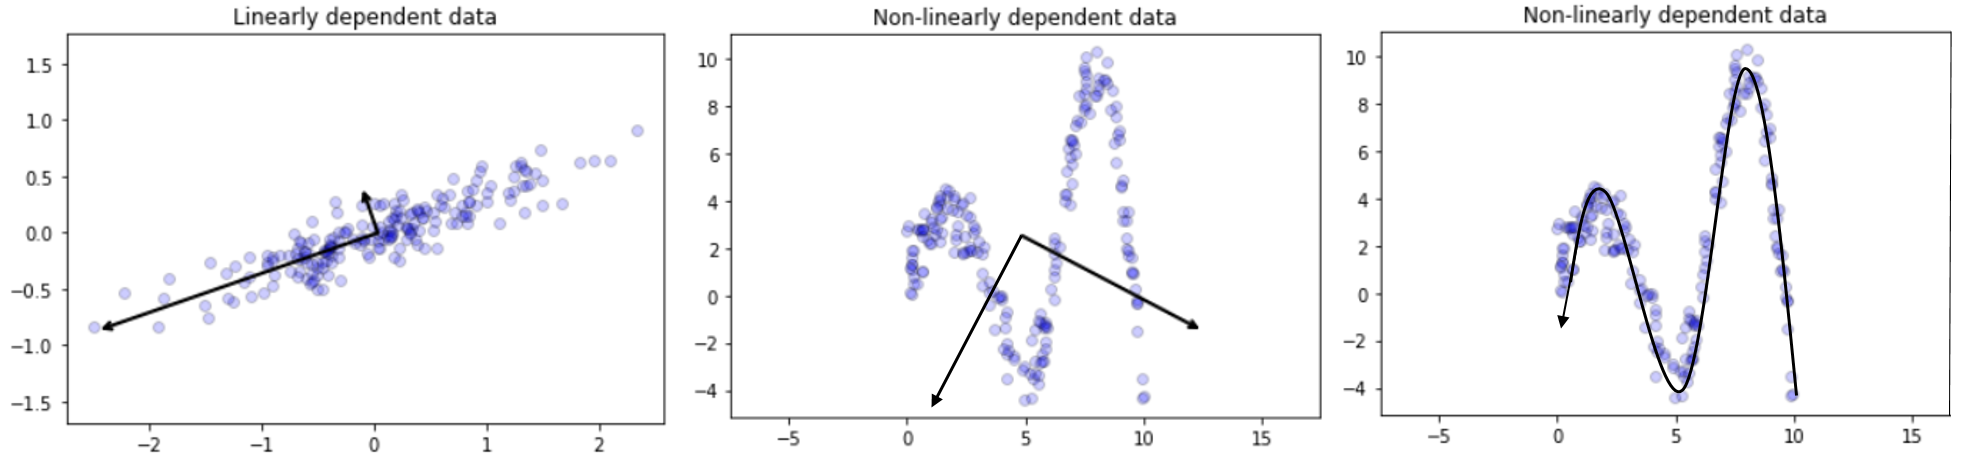
\includegraphics[scale=0.4]{img/pca-linear-separation-demo.png}
		\caption{\label{fig:pca-cons-demo-1}Demonstration of PCA's low performance for non-linearly dependent data}
	\end{figure}
	
	\item Spread maximization. 
	PCA searches for a subspace where projected data has the maximal spread. However, this is not always the best way to represent data in lower-dimension subspace. A common example is the task of separating and counting pancakes from an image (see ~\autoref{fig:pca-cons-demo-2}). Important information for the task (number of pancakes) is located along Z axis which has the lowest variance. So Z axis will be the last principal component identified by PCA which is not what required. 
	
	\begin{figure}[h]
		\centering
		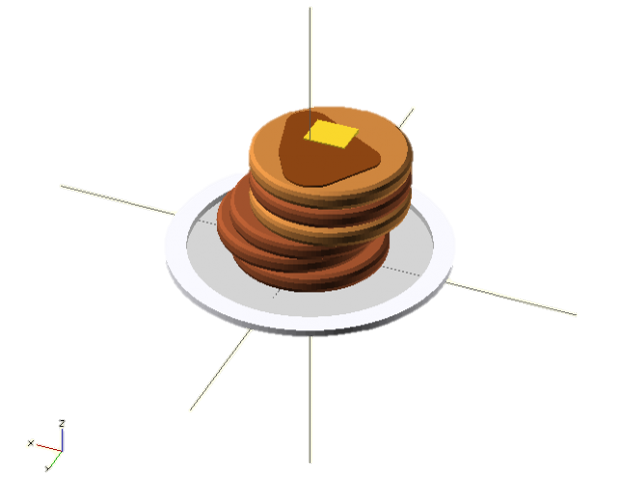
\includegraphics[width=.5\textwidth, scale=0.4]{img/pancakes-white.png}
		\caption{\label{fig:pca-cons-demo-2}Image from  \href{http://golancourses.net/2014/kevan/01/23/3d-parametric-pancakes/}{3D Parametric Pancakes}
		}
	\end{figure}
	
	\item Principal components are hard to interpret.
	PCA reveals implicit dependencies in data which is non-trivial to interpret in case of high-dimensional space reduction. The leverage for this issue is deep understanding of domain.
	
	\item Orthogonality assumptions.
	PCA comes up with orthogonal principal components, which do not overlap in the space. For some tasks such functionality will produce wrong results (see ~\autoref{fig:pca-cons-demo-3}).
	
	\begin{figure}[h]
		\centering
		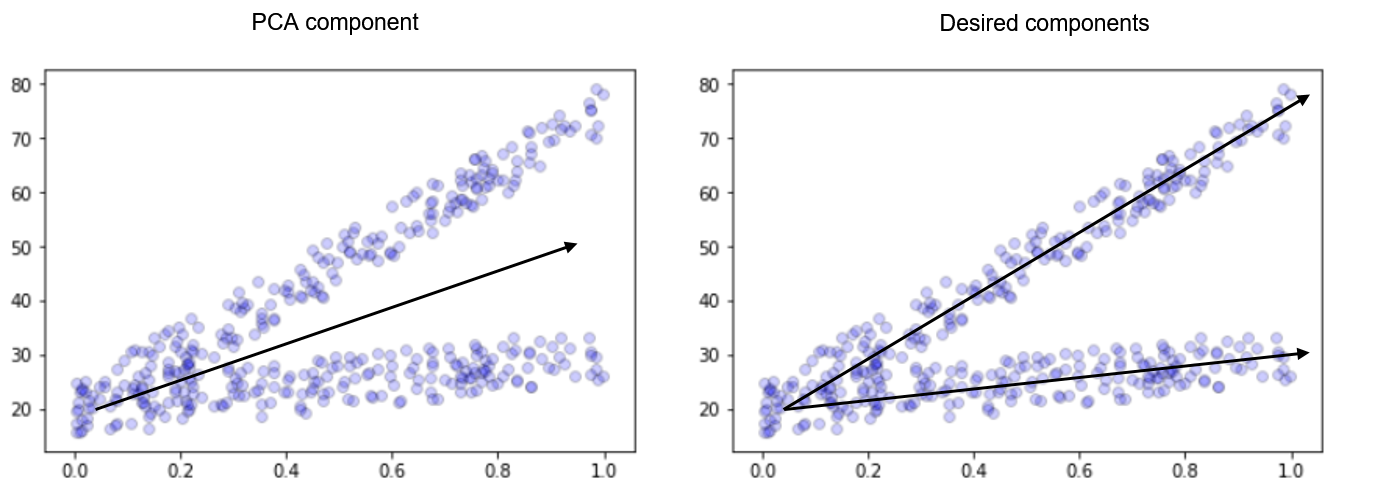
\includegraphics[scale=0.5]{img/non-orthogonal-components.png}
		\caption{\label{fig:pca-cons-demo-3}Demonstration of PCA's low performance for non-linearly dependent data}
	\end{figure}

	\item Outliers and missing data sensitivity.
	We introduced PCA here as eigenvalue decomposition of a data covariance matrix. The latter is highly sensitive to sample outliers and corrupted data (also referred as intra-sample outliers) \citep{shlens}. This raises two issues:
		\begin{enumerate}
			\item PCA is a linear combinations of all input variables whereas in case of corrupted or missing entries presence we need to exclude some incomplete variables.
			
			\item in some contexts, outliers can be difficult to identify. In this case we are unable to remove them in order to get better performance from PCA. Whereas there is a way to overcome the issue by introducing robustness to the algorithm. This will be considered beneath.
		\end{enumerate}
	
	
\end{enumerate}

\section{Modifications of PCA}
Despite the limitations mentioned, PCA is still a powerful method for data analysis, visualization and dimensionality reduction. That is why numerous modifications were developed to overcome its drawbacks and broaden scope of applications. We will provide succinct description of the most common extensions of PCA.

\subsection{Robust PCA}
Gross errors in observations are now ubiquitous in modern applications
such as image processing, web data analysis, and bioinformatics, where some measurements
may be arbitrarily corrupted (due to occlusions, malicious tampering, or sensor failures) or simply irrelevant to the low-dimensional structure we seek to identify with PCA.The best algorithm which deals with data corruption is Robust PCA (RPCA).

Suppose the data under study can naturally be decomposed into low-rank ($L_0$) and sparse ($S_0$) components\footnote{This is not a synthetic requirement and can be done in a number of applications, refer to \citep{cardes} for examples.}:
\begin{equation}
M = L_0 + S_0
\end{equation}

RPCA allows to recover a low-rank matrix $L_0$ from highly corrupted measurements in $M$. Classical PCA works good when the noise term $N_0$ in $M$ is small. In contrast to this $S_0$ can have arbitrarily large magnitude, and their support is assumed to be sparse but unknown \citep{cardes}.


\subsection{Multilinear PCA}
Suppose we need to reduce dimensionality not of a simple matrix $M \in R^2$ but of a n-way array, i.e. a cube or hyper-cube of numbers, also informally referred to as a "data tensor". Common examples of tensor are 2-D/3-D images and video sequences. To deal with tensors PCA is generalized to multilinear PCA (MPCA). MPCA performs feature extraction by determining a multilinear projection that captures most of the original tensorial input variation. The solution is iterative in nature and it proceeds by decomposing the original problem to a series of multiple projection subproblems \citep{lu}. 

MPCA is applied to 3-D object recognition tasks in machine vision, medical image analysis, space-time analysis of video sequences for activity recognition in human-computer interaction, etc.  MPCA is further extended to uncorrelated MPCA, non-negative MPCA and robust MPCA.

\subsection{Nonlinear generalizations}
In real-world problems we often need to work with non-linear dependencies between features in data. For such tasks Hastie and Stuetzle \citep{hastie} proposed bending the loading
vectors to produce curves that approximate the nonlinear relationship between
a set of two variables. Such curves are called principal curves, their multidimensional extensions produce principal surfaces or principal manifolds \citep{gorban}.

Another popular way to use PCA in case of nonlinearity is kernel PCA and rest of the report will be devoted to it.

\section{Kernel Principal Component Analysis}
Kernel principal component analysis, or kPCA, is a nonlinear generalization of PCA using technique of kernel methods, also known as ``kernel trick''. The main idea is to map the original data nonlinearly into a feature space $F$ by 
\begin{equation}
\phi: R^N \rightarrow F 
\end{equation}
and then perform PCA, which implicitly defines nonlinear
principal components in the original data space (see ~\autoref{fig:kpca_bishop}). Even if $F$ has arbitrarily large dimensionality, for certain choices of $\phi$ it is still possible to perform PCA in $F$. This is done by use of kernel functions \citep*{original_paper}.

\begin{figure}[ht]
	\centering
	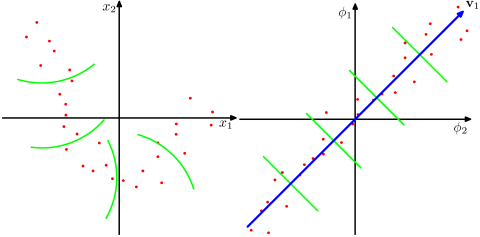
\includegraphics[width=0.7\textwidth]{img/kpca_example_from_bishop.png}
	\caption{\label{fig:kpca_bishop}Kernel PCA. Data set in original data space (left-hand plot) and in the feature space $F$ (right-hand plot). \boldmath$v_1$ is a first principal component obtained in the feature space. Green lines indicate linear projections of data onto \boldmath$v_1$ \citep{bishop}}
\end{figure}


\subsection{Algorithm explanation}
Consider a data set $X$ containing $N$ observations of $D$ features $(D < N)$ and a nonlinear transformation $\phi(x)$ into an $M$-dimensional feature space $F$. For now let us assume that projected data set is centered, so $\dfrac{1}{N}\sum_{n=1}^{N}{\phi(x_n)}=0$.
The $M \times M$ covariance matrix in feature space is given by
\begin{equation}\label{cov_matrix}
C =  \dfrac{1}{N}\sum_{n=1}^{N}{\phi(x_n)\phi(x_n)^T}
\end{equation}

\subsubsection{Eigenvalue equation derivation}
We need to solve the following eigenvalue problem

\begin{equation}\label{eigenvector_eq}
C \bm{v}_i = \lambda_i \bm{v}_i
\end{equation}
%
$i=1,...,M$. Our goal is to solve this equation without working directly in the feature space as due to its size this will be computationally inefficient. Substituting $C$ from (\ref{cov_matrix}) we get
%
\begin{equation}
\dfrac{1} {N} \sum_{n=1}^{N} {\phi(x_n)\{\phi(x_n)^T \bm{v}_i\}} = \lambda_i \bm{v}_i
\end{equation}

Provided $\lambda_i > 0$, the vector $v_i$ is given by a linear combination of the $\phi(x_n)$ and so $\forall\ i \ \exists$ column vector $\bm{\alpha}_i \in R^N$  such that:

\begin{equation}\label{eigenvector_by_alphas}
 \ v_i = \sum_{n=1}^{N}{\alpha_{in}\phi(x_n)}
\end{equation}

Substituting \eqref{cov_matrix} and \eqref{eigenvector_by_alphas} into \eqref{eigenvector_eq}, we obtain

\begin{equation}\label{big_equation}
\dfrac{1}{N}\sum_{n=1}^{N}{\phi(x_n)\phi(x_n)^T} \sum_{m=1}^{N}{\alpha_{im}\phi(x_m)^T} = \lambda_i \sum_{n=1}^{N}{\alpha_{in}\phi(x_n)^T}
\end{equation}

The key thing here is to express last equation in terms of kernel function defined as $k(x_n, x_m) = \phi(x_n)^T\phi(x_m)$. It is done by multiplying both sides by $\phi(x_l)^T$ which results to the next:

\begin{equation}
\dfrac{1}{N}\sum_{n=1}^{N}{k(x_l, x_m)} \sum_{m=1}^{N}{\alpha_{im}k(x_n, x_m)} = \lambda_i \sum_{n=1}^{N}{\alpha_{in}k(x_l, x_m)}
\end{equation}
or in matrix notation
\begin{equation}\label{K_1}
K^2 \bm{\alpha}_i = \lambda_i N K \bm{\alpha}_i
\end{equation}
If we remove a factor of K from both sides we obtain following eigenvalue problem
\begin{equation}\label{K_2}
K \bm{\alpha}_i = \lambda_i N \bm{\alpha}_i
\end{equation}

By solving the problem we find eigenvectors $\bm{\alpha}_i$. Note that solutions of (\ref{K_1}) and (\ref{K_2}) differ only by eigenvectors that correspond to zero eigenvalues of K, hence removing $K$ from both sides of (\ref{K_1}) does not affect principal components.  

\subsubsection{Kernel centering}
So far, we assumed that projected data set has zero mean. But in general it will not be the case. The standard way to centralize data set is to compute mean and then subtract it from every data point.
Here we wish to avoid working in feature space and express everything in terms of kernel function. Let's denote projected data set after centering as $\widetilde{\phi}(x_n)$.

\begin{equation}
\widetilde{\phi}(x_n) = \phi(x_n) - \frac{1}{N}\sum_{l=1}^{N} \phi(x_l)
\end{equation}
and the corresponding elements of the Gram matrix
\begin{equation}
\begin{aligned}
K_{nm} = \widetilde{\phi}(x_n)^T\widetilde{\phi}(x_m) = 
\phi(x_n)^T\phi(x_m) -
\sum_{l=1}^{N}{\phi(x_n)^T\phi(x_l)} - \\ \sum_{l=1}^{N}{\phi(x_l)^T\phi(x_m)} +  \dfrac{1}{N^2}\sum_{j=1}^{N}\sum_{l=1}^{N}{\phi(x_j)^T\phi(x_l)} = \\
k(x_n, x_m) - \sum_{l=1}^{N}{k(x_n, x_l)} - \sum_{l=1}^{N}{k(x_l, x_m)} + \dfrac{1}{N^2}\sum_{j=1}^{N}\sum_{l=1}^{N}{k(x_j, x_l)}
\end{aligned}
\end{equation}
or in a matrix notation
\begin{equation}
\widetilde{K} = K - 1_NK - K1_N + 1_NK1_N
\end{equation}
where $\widetilde{K}$ is centered kernel matrix, $1_N$ is $N \times N$ matrix in which every element equals to $\dfrac{1}{N}$ \citep{bishop}.
So, we are able to evaluate $\widetilde{K}$ using only kernel function.
\subsubsection{Finding principal component projection}
After solving the eigenvalue problem 
$\widetilde{K}\bm{\alpha}_i = \lambda_i N \bm{\alpha}_i$, 
we can find projection onto principal components in terms of the kernel function.
Using (\ref{eigenvector_by_alphas}), projection of a point $x$ onto eigenvector $i$ is given by
\begin{equation}\label{projection_kpca}
\phi(x)^T \bm{v}_i = \sum_{n=1}^{N}{\alpha_{in}\phi(x)^T\phi(x_n)} = \sum_{n=1}^{N}{\alpha_{in}k(x, x_n)}
\end{equation}

Note that neither (\ref{eigenvector_eq})  nor (\ref{projection_kpca}) requires the $\phi(x)$ in explicit form, we only need their dot product to use kernel function without actually performing the map $\phi$ \citep{original_paper}. 

Note that the number of nonzero eigenvalues cannot exceed the number of observations $N$, because
the $M \times M$ covariance matrix in feature space has rank at most $N$ ($N<M$). So, kPCA leads to eigenvector expansion of the $N \times N$ kernel matrix $K$ \citep{bishop}.

\pagebreak
\subsection{Implementation of kPCA}
Main steps of kPCA algorithm:
\begin{enumerate}
	\item Pick up a kernel function;
	\item Construct $M \times M$ dot product kernel matrix $K$ of original data set;
	\item Compute centered kernel matrix $\widetilde{K} = K - 1_N K - K 1_N + 1_N K 1_N$;	\item Solve an eigenvalue problem $\widetilde{K} \bm{\alpha}_i = \lambda_i N \bm{\alpha}_i$;
	\item Compute projections of any point $x$ onto eigenvectors (principal components);
\end{enumerate}
We managed to implement kPCA by ourselves. The source code can be found \href{https://github.com/Irynei/KernelPCA}{here}.

\subsection{Examples of kPCA performance}
Here we want to demonstrate kPCA performance on specific examples.

Consider three centric clouds of points on plane (left-hand plot on ~\autoref{fig:three-centric-circles-2d}). Colors of the points are not known to algorithms and used merely for visualization purposes. As we can see the data is not linearly separable, so standard PCA won't work. Let's now map the data on higher dimension using the (Gaussian) radial basis function kernel, or RBF kernel, defined as

\begin{equation}
	k({x},{y})=e^{{\frac  {-||{x}-{y}||^{2}}{2\sigma ^{2}}}}
\end{equation}
%

As a result in 3-D we obtain a representation as on right-hand plot of ~\autoref{fig:three-centric-circles-2d}.

\begin{figure}[h]
	\centering
	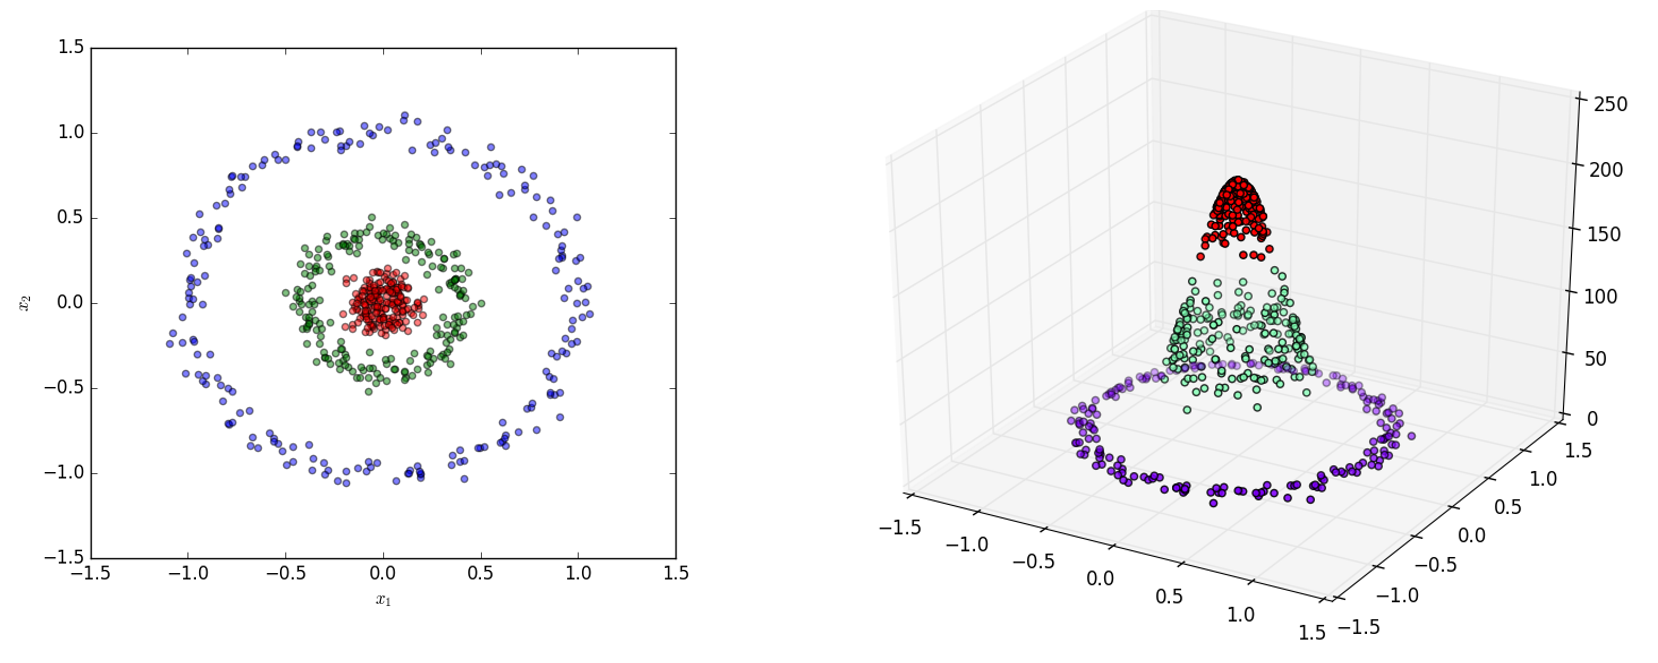
\includegraphics[scale=0.35]
	{img/demo-kpca-1.png}
	\caption{\label{fig:three-centric-circles-2d}Three concentric clouds of points on 2-D and 3-D}
\end{figure}

We can see that in 3-D the points are linearly separable by a hyperplane. This is exactly what kPCA does.

The result of applying kPCA to the initial data set can be seen on left-hand plot of ~\autoref{fig:compare-kpca-pca}. What noticeable is that we can pick out three groups of data merely along the first principal component produced by kPCA.  Whereas linear PCA (right-hand plot on ~\autoref{fig:compare-kpca-pca}) operates only in the given (in our case 2-D) space, in which the concentric point clouds are not linearly separable.

The described capabilities of kernel PCA make it widely applicable in novelty detection \citep{hoffman} and image de-noising \citep{mika}.


\begin{figure}[h]
	\centering
	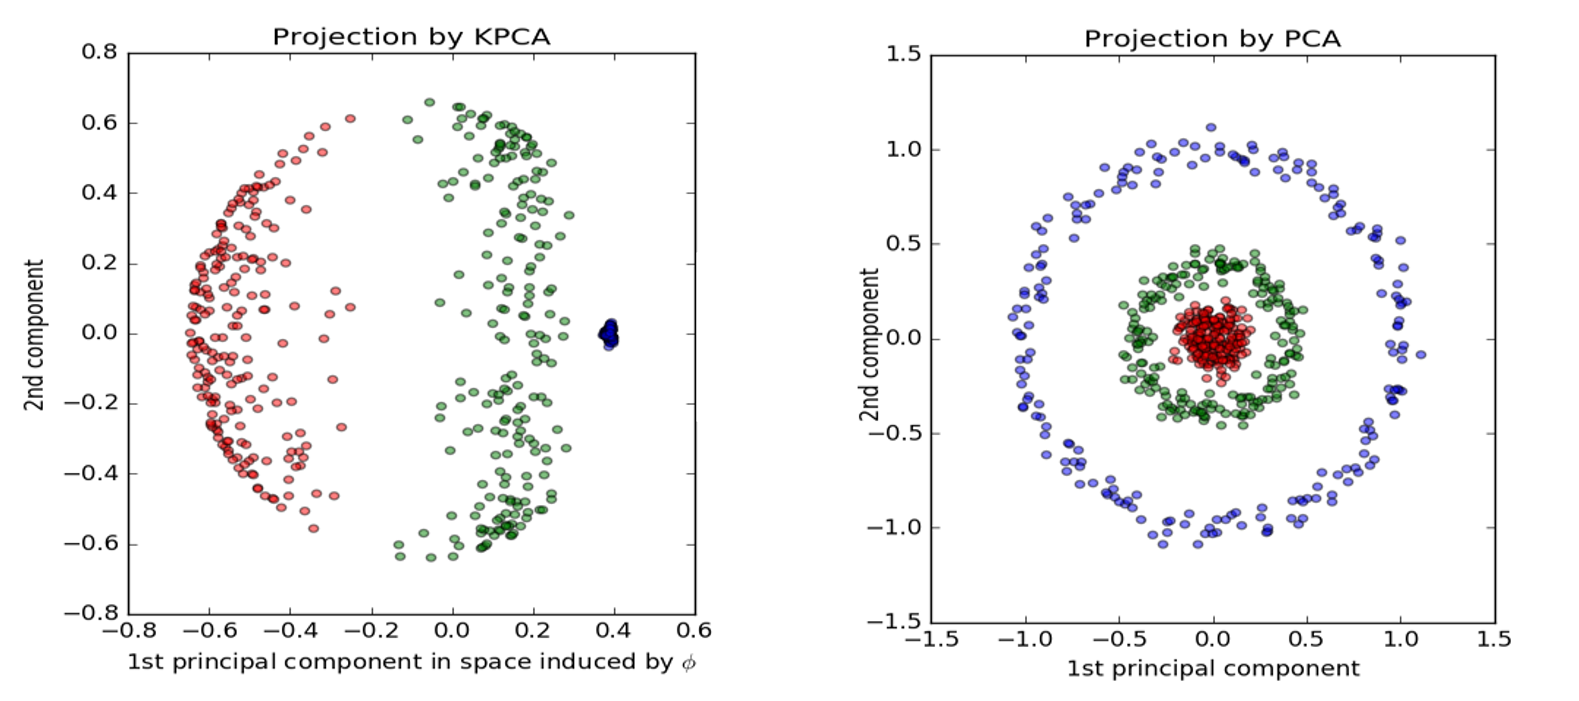
\includegraphics[scale=0.35]
	{img/demo-kpca-2.png}
	\caption{\label{fig:compare-kpca-pca}Comparison of applying PCA and kPCA to three concentric clouds of points}
\end{figure}

\subsection{Pros and cons of kPCA}
Kernel PCA has the next advantages:

\begin{itemize}
	\item able to separate data in nonlinear case;
	\item as PCA, kPCA is an unsupervised method, so the number of principal components does not need to be specified in advance.
\end{itemize}
On the other hand, kPCA has the next drawbacks:

\begin{itemize}
	\item the kernel matrix $K$ is $N \times N$, so in case of big $N$ storing K will be a problem and finding eigenvalues/eigenvectors will be a computationally complex operation. 
	\item as PCA, kPCA is still vulnerable to such issues as outliers, noise and missing data.
\end{itemize}


\section{Summary}
In this project we have studied principal component analysis in details, discussed the areas of its application. We have identified the limitations of linear PCA and its possible modifications to overcome them. Then represented a comprehensive explanation of kernel PCA which extends PCA to non-linearly dependent input data. 

\begin{thebibliography}{9}

\bibitem[Bishop (2009)]{bishop}
 Bishop, Christopher M.\textit{Pattern Recognition and Machine Learning}. Springer, Cambridge, U.K., 2006.

\bibitem[Shlens (2014)]{shlens}
 Shlens, Jonathon. \textit{A Tutorial on Principal Component Analysis}.Google Research, Mountain View, USA, 2014.

\bibitem[Cardes (2009)]{cardes}
 Candes, Emmanuel J.; Li, Xiaodong ; Ma, Yi; Wright, John. \textit{Robust Principal Component Analysis?} J.ACM, 58(11):1-37, 2009 
 
\bibitem[Lu (2008)]{lu} Lu, Haiping; Plataniotis, Konstantinos N.; Venetsanopoulos,  
 Anastasios N. 
 \textit{MPCA: Multilinear Principal Component Analysis of Tensor Objects}.  IEEE Transactions on Neural Networks, 19(1):18-39, 2008
 
\bibitem[Hastie (1989)]{hastie}
 Hastie, Trevor; Stuetzle, Werner. \textit{Principal Curves}. Journal of the American Statistical Association, 84(406): 502-516, 1989.

\bibitem[Gorban (2007)]{gorban}
 Gorban,  Alexander N.; Kegl, Balazs; Wunsch, Donald C.; Zinovyev, Andrei. \textit{Principal Manifolds for Data Visualisation and Dimension Reduction}. Springer, Berlin – Heidelberg – New York, 2007. 

\bibitem[Scholkopf (1998)]{original_paper}
Scholkopf, Bernhard; Smola, Alex; Muller, Klaus-Robert.
\textit{Nonlinear component analysis as a kernel eigenvalue problem.}  Berlin, Germany., 1998.

\bibitem[Hoffman (2007)]{hoffman}
Hoffmann, Heiko.\textit{ Kernel PCA for Novelty Detection}. Pattern Recognition, 40: 863-874, 2007.
 
\bibitem[Mika (1999)]{mika}
Mika, Sebastian; Scholkopf, Bernhard. \textit{Kernel PCA and De-Noising in Feature Spaces}. NIPS, 1999.
\end{thebibliography}

\end{document}